\section{Predictive Analysis}
In this section, we consider the problem of predicting the spending behavior of each customer.We will use the main classifier models and evaluate their performances.

First, we will use the customer profile deriving from the K-means clustering, from the previous section.
From the Figure \ref{fig:skmclust}, we recall that we partitioned the dataset in 3 clusters, that represent the \textbf{high-spending} customers, the \textbf{medium-spending} customers and the \textbf{low-spending} customers.
We can see that the clusters are well separated from each other, and so we can use them as customer classification. 

To perform the task, which is a \emph{supervised} one, we split the dataset into training and test set, equal to the 75\% and 25\% of the dataset respectively. Plus, during the splitting, we specify that each partition must have approximately the same relative class frequencies;
that is to manage the unbalance we have in the original dataset, in which the \textbf{medium-spending} $\Leftarrow$ \textbf{DA CONTROLLARE} customers are much more frequent than the other classes.

For each model, we perform a grid search, to find the best values for some hyperparameters; for that, we used a \emph{K-fold cross validation}, with $K=5$.

\subsection{Support Vector Classifier}
\begin{minipage}{0.6\textwidth}
The first model we analyze is the \textbf{SVM}, that is a classifier that searches for an hyperplane that can linearly separate the data points, possibly in a transformed space, in the non-separable case.

We use a Linear Support Vector Classifier and, after the grid search, we found that the best value for the regularization parameter is $C=1000$.\\
With this configuration, we achieved a training accuracy of 0.9906 and a test accuracy of 0.9962.

From the Figure \ref{fig:svm_confusion}, we can see the confusion matrix related to the results on the test set, and we notice that the model made only 4 mistakes on the whole dataset; for that, we have that also the precision and the recall for each class are all above 0.98.
\end{minipage}
\begin{minipage}{0.4\textwidth}
\centering
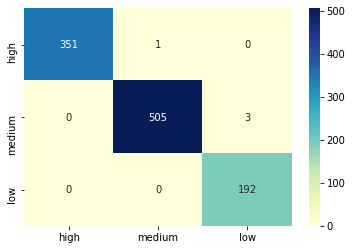
\includegraphics[width=0.90\textwidth]{img/svm_confusion.png}
\captionsetup{justification=centering}
\captionof{figure}{Confusion Matrix\\ for SVM Classifier}
\label{fig:svm_confusion}
\end{minipage}

\subsection{Neural Network}
\begin{minipage}{0.6\textwidth}
Now, we use a Neural Network, in particular a \textbf{Multi Layer Perceptron}.\\
The best values for the hyperparameters that we found was:
\begin{itemize}
\item 1 hidden layer with 50 units
\item Logistic activation function
\item Learning rate equal to 0.001
\item The \emph{lbfgs} optimizer, that can converge faster and with better results on small datasets like ours
\end{itemize}

With this model, we got a training accuracy of 1 and a test accuracy of 0.999; the reason is clear in Figure \ref{fig:nn_confusion}, where we can see that just one data point was misclassified.
\end{minipage}
\begin{minipage}{0.4\textwidth}
\centering
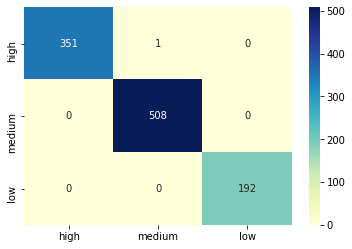
\includegraphics[width=0.90\textwidth]{img/nn_confusion.png}
\captionsetup{justification=centering}
\captionof{figure}{Confusion Matrix\\ for Neural Network}
\label{fig:nn_confusion}
\end{minipage}

\subsection{Naive Bayes Classifier}

\subsection{K-Nearest Neighbors}

\subsection{Decision Tree}

\subsection{Random Forest}
